\documentclass[10pt]{article}
\usepackage{graphicx, fancyhdr, enumerate}
\usepackage{amsmath, amsfonts, color, multicol, mathtools}
\usepackage{blkarray}

\setlength{\topmargin}{-.55 in} 
\setlength{\textheight}{9 in}
\setlength{\textwidth}{6.625 in} 
\setlength{\evensidemargin}{-.0625 in}
\setlength{\oddsidemargin}{-.0625 in} 
\setlength{\parindent}{0 in}
\setlength{\headheight}{18.0pt}
\newcommand{\ds}{\displaystyle}
\newcommand{\xbar}{\overline{X}}

\DeclarePairedDelimiter{\ceil}{\lceil}{\rceil}

\cfoot{\thepage} 
\renewcommand{\headrulewidth}{0.4pt} 
\renewcommand{\footrulewidth}{0pt} 
\newcommand{\ansfont}[1]{{\textcolor{blue}{\textbf{Answer:}}\ \ #1}}


\lhead{\Large\sffamily Stat 330 (Fall 2016): Homework 3} 
\rhead{\sffamily Due: September 14, 2016}

% Uncomment the following line to remove answers, and comment line out to show answers:
\renewcommand{\ansfont}[1]{}


\begin{document}
\pagestyle{fancy} 
Show all of your work, and \emph{please} staple your assignment if you use more than one sheet. Write your name, the course number and the section on every sheet. 

\begin{enumerate} 
    \item (Baron's book): 2.16
    
    \ansfont{
      \newline
      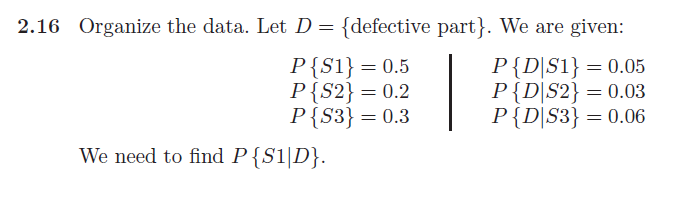
\includegraphics[width=13cm]{baron2-16_1}
      \newline
      \hspace*{1cm}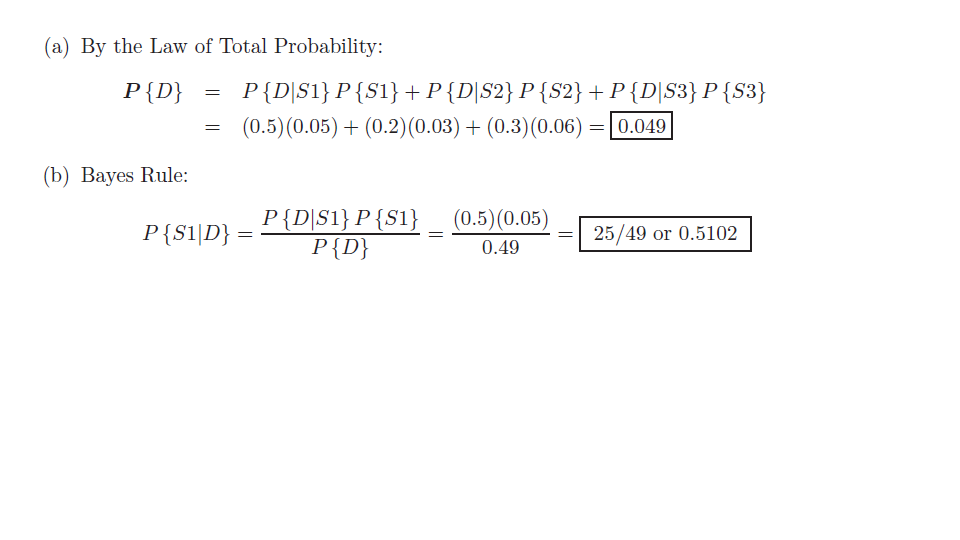
\includegraphics[width=11cm]{baron2-16_2}
    }
    
    
  \item Imagine that we are sending information across some sort of ``noisy channel'' (say, a network), where each bit we transmit randomly ``flips'' with probability $p$, independently of other bits that are sent, while moving across the channel to the receiver. This sort of situation corresponds to what is called a \emph{binary symmetric channel}:
\begin{figure}[h]
\begin{center}
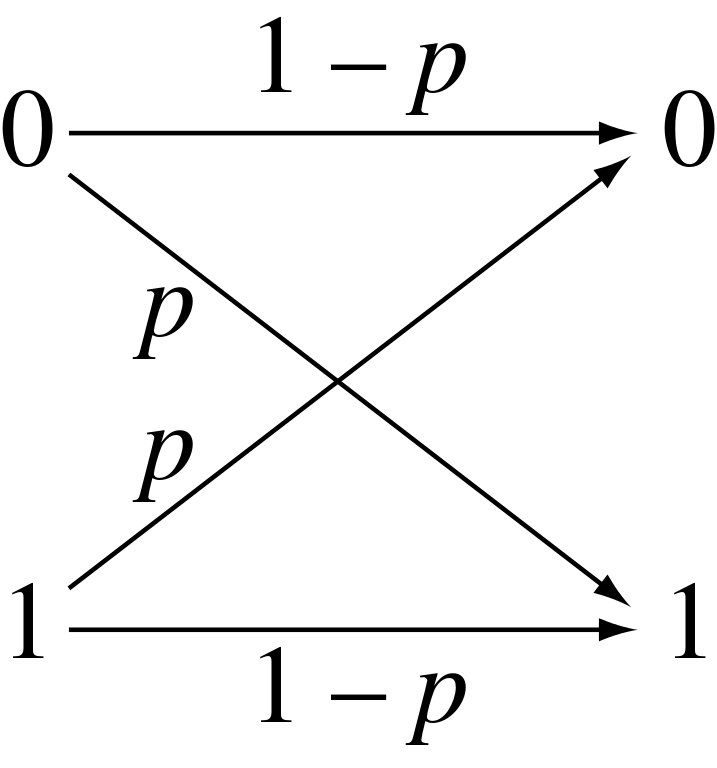
\includegraphics[height = 1in, width = 1in]{Binary_symmetric_channel.png}
\caption{A binary symmetric channel with error probability $p$.}
\end{center}
\end{figure}

Suppose that in order to reduce the rate of transmission errors, we first replicate each bit we want to send 3 times, and that the receiver takes each block of 3 bits received and determines that the original bit was a $1$ if at least $2$ of the bits in the block are $1$'s, and $0$ otherwise. That is, there might be a situation where the sender wants to transmit a $0$, so he first replicates this bit three times to get $000$, and sends each of these bits over the channel one at a time. The receiver may receive the string $010$ (the middle bit was flipped by the channel) and deduce that the bit intended to be sent was a $0$. The entire process looks like:
\[ 0 \to 000 \to 010 \to 0 \]
Where the steps are, in order ``encoding'', ``transmission'', and ``decoding''. This encoding scheme is called a ``repitition code'', and the decoding algorithm is called the ``majority vote algorithm'' for obvious reasons.

\vspace{.1in}
\begin{enumerate}
  \item Suppose the next bit in the message is a $0$, and that this is encoded and sent over the channel as described above. How many possible bit strings can the receiver receive, and what is the probability (in terms of $p$) of each one?
  \item What changes if the next bit in the message is a $1$ rather than a $0$? Answer verbally or with a list of probabilities.
  \item How many ways can we receive a 3-bit block with $k$ errors ($k$ flipped bits)? For a given $k$, is the probability of receiving each of these strings the same or different?
  \item What is the probability that after the decoding process ($010 \to 0$ in the above example) that the decoded bit differs from the one that was intended to be sent?
  \item If we generalize this communication scheme and replicate each new bit $n$ times instead of 3, for odd $n$, what is the probability that the decoded bit differs from the one that was intended to be sent?
  \item Suppose that bits being sent are a 50-50 split between 0 and 1. If you receive a 010, what is the probability the sender sent a 0?
\end{enumerate}

% SOLUTION
\ansfont{
\begin{enumerate}
\item There are $2^3 = 8$ possible strings. If $x$ represents the number of 1's in the string, then the probability is $\binom{3}{x}p^x(1 - p)^{3 - x}$.
\item The same formula, except $x$ now represents the number of 0's.
\item $\binom{3}{k}$ ways. For a given $k$, these probabilities are all the same.
\item If there are at least two errors, the decoded bit will be wrong, so the probability is $\sum_{x = 2}^3\binom{3}{x}p^x(1 - p)^{3 - x}$.
\item Let $K = \ceil*{\frac{n}{2}}$. Then the probability is $\sum_{x = K}^n\binom{n}{x}p^x(1 - p)^{n - x}$. This inutuitively corresponds to the probability of having a ``majority vote'' in the ``election'' between 0 and 1.
\item Let $T$ represent the true state and $R$ represent the received transmission. We know $P(T=0)=P(T=1)=0.5.$ Then 
\[ \begin{array}{rl}
P(T=0|R=010) &= \frac{P(R=010|T=0)P(T=0)}{P(R=010|T=0)P(T=0)+P(R=010|T=1)P(T=1)} \\
&= \left[1+\frac{P(R=010|T=1)}{P(R=010|T=0)}\frac{P(T=1)}{P(T=0)}\right]^{-1} \\
&= \left[1+\frac{p^2 (1-p)}{(1-p)^2 p }\right]^{-1} \\
&= \left[1+\frac{p}{1-p}\right]^{-1} = 1-p \\
\end{array} \]
\end{enumerate}
}

\item Let $X$ be a random variable with image $Im(X)= \{0,1,2,3\}$.
	\begin{enumerate}
	\item Fill in the blank in the table below to make it a valid probability mass function:
	\[
	\begin{array}{l@{\extracolsep{.1in}}|cccc}
	x & 0 & 1 & 2 & 3 \\ \hline
	p_X(x) & 0.5 & 0.25 & 0.1 & \\
	\end{array}
	\]
	\item Derive the cumulative distribution function for $X$ and draw it in a table. 
	\item Determine the probabilities that... 
		\begin{enumerate}
		\item $X$ is at least 2.
		\item $X$ is neither 0 nor 2.
		\item $X$ is non-negative.
		\end{enumerate}
	\item Find the expected value and variance of $X$.
	\item Let $Y$ be a random variable with $Y = 5-2X$ where X has the $pmf$ from above;
		\begin{enumerate}
		\item Determine the image of $Y$. 
		\item Using the rules for computing expected values and variances of a linear function of a random variable, find the expected value and variance of $Y$
		\end{enumerate}
	\item Suppose we have a collection of independent and identically distributed $X_i$ according to a) and $Z=\sum_{i=1}^n X_i$.
	
		\begin{enumerate}
	 \item What is $E[Z]$?
	 \item What is $Var[Z]$? (Hint: the solution will depend on $n$.)
	 \end{enumerate}
	\end{enumerate}

\ansfont{
	\begin{enumerate}
	\item Since the sum of the probabilities has to be 1 for a probability mass function, $p_X(3) = 1- 0.5-0.25-0.1 = 0.15$.
	\item 
	\[
	\begin{array}{l@{\extracolsep{.1in}}|cccc}
	x & 0 & 1 & 2 & 3 \\ \hline
	p_X(x) & 0.5 & 0.25 & 0.1 & 0.15 \\
	F_X(x) & 0.5 & 0.75 & 0.85 & 1 \\
	\hline
	\end{array}
	\]
	\item 
		\begin{enumerate}
		\item $P(X\ge2) = 1-P(X<2) = 1-P(X\le 1) = 1- 0.75=0.25$ or, equivalently $P(X\ge 2) = P(X=2)+P(X=3) = 0.1+0.15=0.25.$
		\item $P(X\neq 0,2) = 1- P(X=0) - P(X=2)  = 1 - 0.5 - 0.1 = 0.4$
		\item $P(X \ge 0) = 1$
		\end{enumerate}
	\item $E[X] = 0 \cdot P(X=0) + 1 \cdot P(X=1) + 2 \cdot P(X=2) + 3 \cdot P(X=3) = 0 + 0.25 + 0.2+0.45 = 0.9$. To find the variance, we will use the formula $Var[X] = E[X^2]-(E[X])^2$. 
	\[ E[X^2] = 0 \cdot P(X=0) + 1 \cdot P(X=1) + 4 \cdot P(X=2) + 9 \cdot P(X=3) = 0 + 0.25 + 0.4+1.35 = 2 \]
and therefore $Var[X] = E[X^2] - \left( E[X] \right)^2 = 2 - 0.9^2 = 1.19$.
	\item Since $X$ has image $Im(X) = \{0,1,2,3\}$, the image of $Y$ has to be $Im(Y) = \{ 5, 3, 1, -1\}$.
	\item $Y$
	\begin{enumerate}
	\item $E[Y] = E[5-2X] = 5 - 2 E[X] = 5 - 1.8 = 3.2$
	\item $Var[Y] = Var[5 - 2 X] = Var[-2X] = (-2)^2 Var[X] = 4 \cdot1.19 = 2.38$
	\end{enumerate}
	\item $Z$
		\begin{enumerate}
	\item Expectation
	\begin{align*}
	E[Z] &= E\left[ \frac{1}{n} \sum_{i=1}^n X_i \right] \\
	&= \frac{1}{n} \sum_{i=1}^n E[X_i] = \frac{1}{n} n (0.9) = 0.9
	\end{align*}
	\item Variance
	\begin{align*}
	Var[Z] &= Var\left[ \frac{1}{n} \sum_{i=1}^n X_i \right] \\
	&= \frac{1}{n^2} \sum_{i=1}^n Var[X_i] = \frac{1}{n^2} n (1.19) = 1.19/n
	\end{align*}
	\end{enumerate}
	\end{enumerate}
}

\item On average, 8\% of circuit boards are defective.
  \begin{enumerate}
    \item What is the probability of finding exactly 2 defective boards in a batch of
  10 randomly chosen circuit boards?
    \item What is the probability of finding at most 2 defective boards in a batch of
  10 randomly chosen circuit boards?
    \item What is the probability of finding more than 1 but less than 4 defective
      boards in a batch of
  10 randomly chosen circuit boards?
    \item What is the probability that we have to test at least 3 circuit boards to find the first defective one?
    \end{enumerate}

    \ansfont{
      \begin{enumerate}
        \item Let $X$ be the number of defective circuit boards in a sample of size 10.
          Assume that the probability of getting a defective is the same for any circuit board
          and each board is independent of each other to be defective.
          Then $X$ follows a binomial distribution with $n=10$ and $p=0.08$.
          The required probability is
          \begin{align*}
            P(X=2) = {10 \choose 2} 0.08^2 (1-0.08)^{10-2}=0.1478.
            \end{align*}
          \item
          \begin{align*}
            P(X\le2) &= P(X=0) + P(X=1) + P(X=2)\\
            &= {10 \choose 0} 0.08^0 (1-0.08)^{10-0} + {10 \choose 1} 0.08^1
            (1-0.08)^{10-1} + {10 \choose 2} 0.08^2 (1-0.08)^{10-2}\\
            &= 0.9599
            \end{align*}
          \item
            \begin{align*}
            P(1<X < 4) &= P(X=2) + P(X=3)\\
            &= {10 \choose 2} 0.08^2 (1-0.08)^{10-2} + {10 \choose 3} 0.08^3 (1-0.08)^{10-3}\\
            &= 0.1821
            \end{align*}
          \item Let $Y$ be the number of circuit boards tested to find the first defective one.
          Assume that the probability of getting a defective is the same for any circuit board
          and each board is independent of each other to be defective.
          Thus $Y$ follows a Geometric distribution with $p=0.08$. There are
          two ways to get the required probability:
          \begin{itemize}
            \item
          \begin{align*}
            P(Y\ge 3) &= 1- P(Y <3)\\
            &= 1- P(Y\le 2)\\
            &= 1- [1- (1-0.08)^2] = 0.8464
          \end{align*}
          since $P(Y\le t) = 1-(1-p)^t$ is the cdf of the Geometric distribution.
        \item 
          \begin{align*}
            P(Y\ge 3) = P(\mbox{the first two boards are not defective}) = (1-0.08)^2 = 0.8464
          \end{align*}
        \end{itemize}
        \end{enumerate}
    }


\item On average, a particular web page is accessed 10 times an hour. Let $X$ be the number of times this web page will be accessed in the next hour.

\begin{enumerate}
\item Of the discrete distributions you have learned, which one is the most suitable for modeling $X$? (Hint: it means \emph{fish} in French.)
\item What is $E[X]$ and $Var[X]$?
\item What is the probability there is at least one access in the next hour?
\item What is the probability there are between 8 and 12 (inclusive) accesses in the next hour?
\item (Bonus) On average, one out of 10 access results in a purchase. What is the distribution for the number of purchases in the next hour? (Hint: you cannot have more purchases than accesses.) 
\end{enumerate}


\ansfont{
  \begin{enumerate}
    \item Poisson
    \item 10 accesses and 10 accesses$^2$
    \item $P(X>0) = 1-P(X=0) = 1-\frac{10^0 e^{-10}}{0!} \approx 1$
    \item $P(8\le X \le 12) = \sum_{x=8}^12 \frac{10^x e^{-10}}{x!} \approx 0.57$.
    \item (Bonus) Let $Y$ represent the number of purchases. Then $Y\sim Bin(X,0.1)$. Using the probability mass functions, we have 
    \[ \begin{array}{rl}
    P(Y=y) &= \sum_{x=0}^\infty P(Y=y,X=x) \\
    &= \sum_{x=y}^\infty P(Y=y|X=x)P(X=x) \\
    &= \sum_{x=y}^\infty {x\choose y} 0.1^y(1-0.1)^{x-y} \frac{10^xe^{-10}}{x!} \\
    &= 0.1^y e^{-10} \sum_{x=y}^\infty \frac{x!}{(x-y)!y!} (1-0.1)^{x-y} \frac{10^x}{x!} \\
    &= \frac{0.1^y e^{-10}}{y!} \sum_{x=y}^\infty \frac{1}{(x-y)!} (1-0.1)^{x-y} 10^x \\
    &= \frac{0.1^y e^{-10}}{y!} \sum_{r=0}^\infty \frac{1}{r!} (1-0.1)^{r} 10^{r+y} \\    
    &= \frac{0.1^y e^{-10}}{y!} \sum_{r=0}^\infty \frac{1}{r!} (1-0.1)^{r} 10^r 10^{y} \\
    &= \frac{1^y e^{-10}}{y!} \sum_{r=0}^\infty \frac{1}{r!} 9^r \\
    &= \frac{1^y e^{-10}}{y!} e^9 \\
    &= \frac{1^y e^{-1}}{y!}
    \end{array} \]
Thus $Y\sim Po(1)$. (Note: the summation is over values $x=y$ because we cannot have more purchases than access and thus $P(Y=y,X=x)$ for $x<y$ are zero.)
  \end{enumerate}
}

    \item (Baron's book): 3.15
    
    \ansfont{
      \newline
      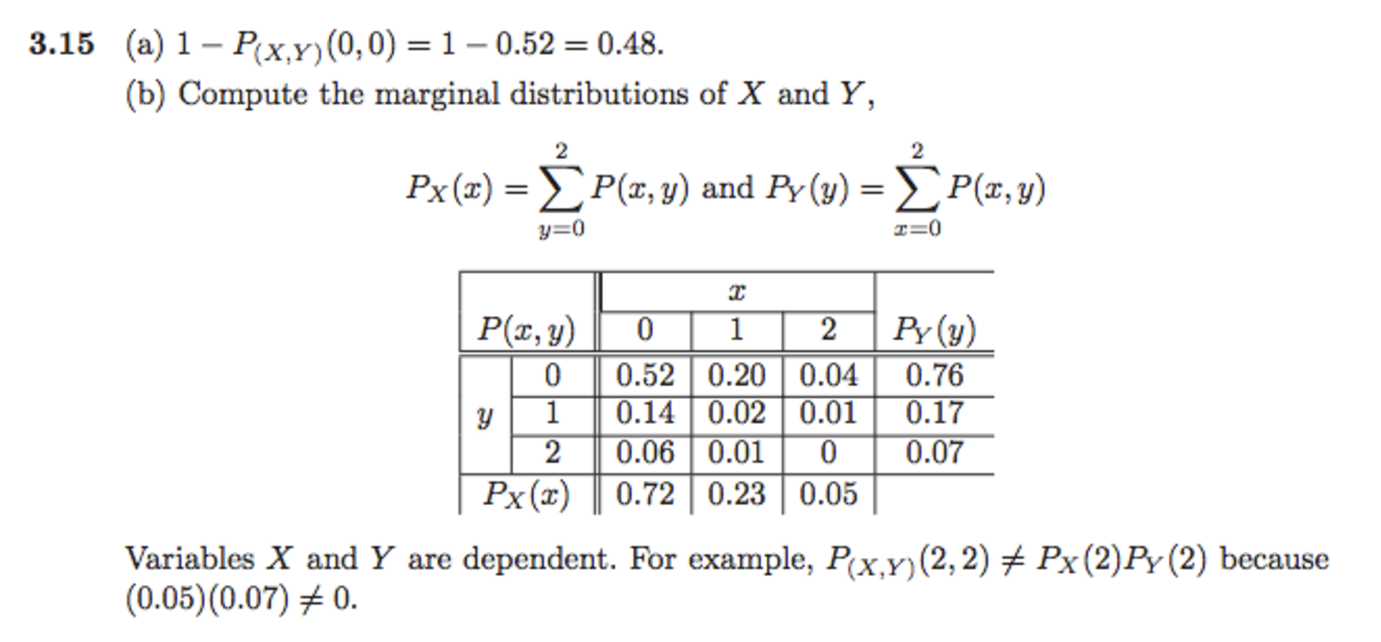
\includegraphics[width=13cm]{baron3-15}
    }
  
\end{enumerate}
\end{document}
